\chapter{Data Analysis}
Data is a crucial part of this project, sourced from various publicly available and directly engaged methods to study the evolution of place names accompanying the transformation of Edo into Benin City. The main data sources used include old and current maps, historical documents accessible through online repositories, structured interviews with local historians and community leaders, surveys distributed to gather contemporary perspectives on historical place names, and integration with publicly available APIs such as OpenStreetMap. Additionally, direct engagement with local communities provided oral histories and traditional knowledge about place names.

Due to the limited availability of public datasets in Nigeria, alternative strategies, such as sourcing historical documents and conducting text analysis, were employed. This approach provided valuable insights despite the data gap.

\section{Analysis of Historical Documents}

Historical documents have been instrumental in unraveling the historical evolution of place names in Edo and Benin City. Analyzing historical documents, maps, and administrative records has highlighted colonial renaming initiatives and their motivations. Indigenous sources, such as oral histories, provided additional perspectives on naming practices. Additionally, the development of a data model and an information system facilitated the management of place name data, including recorded pronunciations.

\subsection{Sources of Data and Processing}

Data collection for this study includes research from publicly available internet sources that incorporate historical documents and chronicles and dialogues with locals to gather perspectives on historical place names. The information that was collected from local historians was later validated by community leaders. Later on, these multiple data sources were processed using data mapping and schema alignment techniques to create a single data model. A custom API was integrated to the web system, ensuring structured data in retrieval and new entries. Manual data entry from authorized users was facilitated through easy-to-use interfaces with validation rules to ensure accuracy and consistency. Bulk data import involved uploading CSV and Excel files from libraries and local post offices, mapping the data to the database schema, and converting data types appropriately.

\textbf{The Benin Kingdom Document:}
This document provides an analysis based on the RAFBookletYear-5-1 \href{https://denhamgreenacademy.e-act.org.uk/wp-content/uploads/sites/5/2020/10/RAFBookletYear-5-1Benin-Kingdom-paper-size-297x21-cmUPDATED.210187322-wecompress.com_.pdf}{Benin-Kingdom} and offers significant insights into the historical, cultural, and socio-economic aspects of the Benin Kingdom.

The document outlines the establishment of the Benin Kingdom, highlighting significant events, key rulers, and cultural practices that shaped its history. It explores key terms such as "Oba" (king or chief), "Ogisos" (first kings of Benin), "Voodoo" (a religion widely followed in Benin), and "Animism" (belief in non-human spirits or souls), shedding light on the religious and social practices prevalent among the Benin people. A detailed timeline of events documents the chronological development of the Benin Kingdom, including the construction of the moat, reigns of notable rulers such as Oba Ewuare the Great, and interactions with European entities like the Portuguese.

The document discusses various geographical locations such as Edo, Ubinu (Benin in Portuguese), and Igodomigodo, providing insights into the territorial expansion and historical evolution of the kingdom. Economic aspects are highlighted through references to "Cowrie shells" used as currency and the establishment of trading links with Europeans, illustrating the kingdom's active participation in regional and international trade networks. Insights into the social structure and political dynamics are provided through mentions of guilds and civil wars, indicating the organizational framework of craftsmen and the internal conflicts within the kingdom. The document serves as an educational resource, offering foundational knowledge about the history, culture, and geography of the Benin Kingdom, particularly targeted at Year 5 students.


\subsubsection{Key Findings}

The tables below summarize key findings based on the text analysis of a historical document. See Table~\ref{tab:vocabulary} for vocabulary terms and their meanings, Table~\ref{tab:timeline} for a timeline of events, and Table~\ref{tab:edo_vocab} for some specific Edo vocabulary.

\begin{table}[htb]
\centering
\caption{Vocabulary of common terms\protect\footnotemark}
\label{tab:vocabulary}
\begin{tabularx}{\linewidth}{|l|X|}
\hline
\textbf{Word} & \textbf{Meaning} \\
\hline
Oba & A king, or chief. \\
\hline
Ogisos & The first kings of Benin. Ogisos means “Rulers of the Sky”. \\
\hline
Empire & Lots of countries or states, all ruled by one monarch or single state. \\
\hline
Guild & A group of people who all do the same job, usually a craft. \\
\hline
Animism & A religion widely followed in Benin. \\
\hline
Voodoo & The belief that non-human objects have spirits or souls. They are treated like Gods. \\
\hline
Cowrie shells & A sea shell which Europeans used as a kind of money to trade with African leaders. \\
\hline
Civil war & A war between people who live in the same country. \\
\hline
Moat & A long trench dug around an area to keep invaders out. \\
\hline
\end{tabularx}
\end{table}

\begin{table}[htb]
\centering
\caption{Timeline of Events\protect\footnotemark}
\label{tab:timeline}
\begin{tabularx}{\linewidth}{|l|X|}
\hline
\textbf{Year} & \textbf{Event} \\
\hline
900 CE & Lots of villages join together and make a kingdom known as Igodomigodo, ruled by Ogisos. \\
\hline
900-1460 CE & A huge earthen moat was constructed around the kingdom, stretching 16,000 km long. \\
\hline
1180 CE & The Oba royal family take over from the Osigo, and begin to rule the kingdom. \\
\hline
1440 CE & Benin expands its territory under the rule of Oba Ewuare the Great. \\
\hline
1470 CE & Oba Ewuare renames the kingdom as Edo, with its main city known as Ubinu (Benin in Portuguese). \\
\hline
1485 CE & The Portuguese visit Edo and Ubinu. \\
\hline
1514 CE & Oba Esigie sets up trading links with the Portuguese, and other European visitors. \\
\hline
1700 CE & A series of civil wars within Benin lead to colonization. \\
\hline
\end{tabularx}
\end{table}

\begin{table}[htb]
\centering
\caption{Some Edo-related terms\protect\footnotemark}
\label{tab:edo_vocab}
\begin{tabularx}{\linewidth}{|l|X|}
\hline
\textbf{Term} & \textbf{Definition} \\
\hline
Edo & A member of a people inhabiting the district of Benin in Nigeria. \\
\hline
Igodomigodo & The historical name of the now fallen Benin Empire. \\
\hline
Ogisos & The first kings of Benin. Ogisos means “Rulers of the Sky.” \\
\hline
Oba & A king or chief. \\
\hline
Empire & Lots of countries or states, all ruled by one monarch or single state. \\
\hline
Kingdom & Over a thousand years ago, a group of people known as the Edo lived in West Africa. Around the year 900, the Edo began to cut down trees and make clearings in the rainforests. Lots of villages joined together to make a kingdom known as Igodomigodo, which was ruled by a series of kings, known as the Ogisos or “Rulers of the Sky”. \\
\hline
Voodoo & A religion widely followed in Benin. It combines elements of Roman Catholic ritual with traditional African magical and religious rites. \\
\hline
Animism & The belief that non-human objects have spirits or souls. \\
\hline
\end{tabularx}
\end{table}

\footnotetext{Data for tables \ref{tab:vocabulary}, \ref{tab:timeline}, and \ref{tab:edo_vocab} sourced from \href{https://denhamgreenacademy.e-act.org.uk/wp-content/uploads/sites/5/2020/10/RAFBookletYear-5-1Benin-Kingdom-paper-size-297x21-cmUPDATED.210187322-wecompress.com_.pdf}{Denham Green Academy}.}

\vspace{0.5cm}
\textbf{Ancient Chronicles:} The investigation of ancient chronicles, such as the "Ife Chronicles" and the "Benin Chronicles," offered foundational accounts of early settlements, legendary narratives, and dynastic histories ~\cite{otterbein1966}. According to these chronicles, early settlements were established by legendary figures imbued with divine or semi-divine attributes, signifying their foundational roles in shaping the social and political landscapes of Edo/Benin City. Legendary narratives recount the exploits of these mythical progenitors, depicting their interactions with supernatural beings, the establishment of kinship ties, and the founding of sacred sites. Dynastic histories trace the lineage of ruling families and the succession of kingship within the Edo/Benin polity, highlighting key moments of political consolidation, territorial expansion, and cultural innovation. Through a blend of historical fact and mythic symbolism, these chronicles offer insights into the deep-rooted traditions and cultural heritage underpinning the identity of Edo/Benin City.


\vspace{0.5cm}
\textbf{Ancient Chronicles:} The investigation of ancient chronicles, such as the "Ife Chronicles" and the "Benin Chronicles," offered foundational accounts of early settlements, legendary narratives, and dynastic histories ~\cite{otterbein1966}. According to these chronicles, early settlements were established by legendary figures imbued with divine or semi-divine attributes, signifying their foundational roles in shaping the social and political landscapes of Edo/Benin City. Legendary narratives recount the exploits of these mythical progenitors, depicting their interactions with supernatural beings, the establishment of kinship ties, and the founding of sacred sites. Dynastic histories trace the lineage of ruling families and the succession of kingship within the Edo/Benin polity, highlighting key moments of political consolidation, territorial expansion, and cultural innovation. Through a blend of historical fact and mythic symbolism, these chronicles offer insights into the deep-rooted traditions and cultural heritage underpinning the identity of Edo/Benin City.

\textbf{Colonial Records:} The colonial era ushered in a new era of documentation, with European explorers, missionaries, and administrators recording detailed observations of indigenous societies and governance structures. Archival collections housed in national archives and colonial repositories, including the National Archives of Nigeria and the British Library, yielded valuable correspondence, reports, and surveys shedding light on colonial encounters and administrative reforms in the Edo/Benin region ~\cite{oliver1985}.

\textbf{Travelogues and Expedition Accounts:} Travelogues and expedition accounts penned by explorers, traders, and ethnographers provided firsthand descriptions of landscapes, settlements, and cultural practices in the Edo/Benin hinterlands. Notable works such as Richard Burton's "A Mission to Gelele, King of Dahomey" and Mary Kingsley's "Travels in West Africa" offered vivid portrayals of local customs, traditions, and historical landmarks ~\cite{burton2011} and ~\cite{kingsley1988}.

\textbf{Archaeological Reports:} The rich archaeological heritage of Edo/Benin City yielded a wealth of material culture and stratigraphic data, as documented in archaeological reports and excavation findings. Reports from pioneering archaeologists such as Thurstan Shaw, Graham Connah, and Ekpo Eyo provided crucial insights into ancient Benin's material culture, settlement patterns, and technological advancements ~\cite{shaw1970,connah1975}. Shaw's 1979 report delved into excavations, revealing evidence of urban planning, architectural structures, and material culture indicative of a burgeoning city. Connah's work from 1975 focused on settlement patterns, technological innovations, and social organization within ancient Benin, shedding light on the processes that contributed to its urbanization. Eyo's report from 1980 provided insights into the stratigraphic data and chronological sequence of cultural developments in the region, offering valuable context for understanding the transition from Edo to Benin City. These archaeological findings collectively contribute to our understanding of the socio-cultural and economic dynamics accompanying the city's transformation over time.

\textbf{Oral Traditions and Indigenous Knowledge:} Recognizing the importance of oral traditions as repositories of collective memory and cultural heritage, local communities and indigenous scholars documented oral histories, folk tales, and place-name traditions associated with Edo/Benin City. Transmitted across generations, these narratives offered nuanced perspectives on the socio-cultural dynamics shaping the toponymic landscape. One oral tradition recounted by local communities involved narratives of migration, conquest, and settlement that contributed to the transformation of Edo into Benin City. For instance, stories of legendary figures or ancestral rulers who led their people to establish a new capital marked the beginning of Benin City's emergence as a prominent political and cultural center. These tales provided insights into the socio-political processes, power struggles, and symbolic meanings associated with the city's renaming and evolution.

\section{Main Outcomes}

The analysis highlighted significant colonial impacts on place naming practices. Colonial authorities often imposed English or European names on geographical features, urban centers, and administrative districts. Despite these changes, indigenous place names persisted in local memory and oral traditions, serving as resilient symbols of cultural heritage and identity. The dynamic nature of place naming practices was evident, with linguistic diversity, cultural influences, and historical legacies playing a crucial role in shaping place names. These findings illustrate the multifaceted nature of place naming practices in Edo and Benin City and contribute to a deeper appreciation of the region's cultural heritage and identity.

\section{Visualization of Place Name Evolution}

Utilizing Geographic Information System (GIS) technology, the evolutionary journey of Edo to Benin City was visualized through maps and charts. These visualizations offer a spatial-temporal perspective on the transformation of toponyms over centuries, shedding light on the complex processes and historical events that shaped the city's nomenclature.

These visualizations facilitate various types of analyses using the collected data. Spatial analysis through charts and heatmaps can identify geographical patterns and regional influences on place naming practices. Temporal analysis using histograms allows researchers to trace the historical trajectory of place names, identifying significant periods of change or continuity. Network analysis offers insights into the connectivity and relationships between different place names, revealing underlying social or cultural networks. Word clouds can uncover common linguistic or cultural themes in naming practices. Overall, these visual tools enhance the understanding of the historical and socio-cultural dimensions of place name evolution, aiding in the preservation and study of cultural heritage.

A number of visualizations with geocoded data were performed to gain further insights into the spatial distribution and patterns of historical place names. The heatmap visualization allows the density or concentration of historical place names in different areas to be seen, helping identify areas with high concentrations of place names and sparsely populated areas.

\begin{figure}[H]
    \centering
    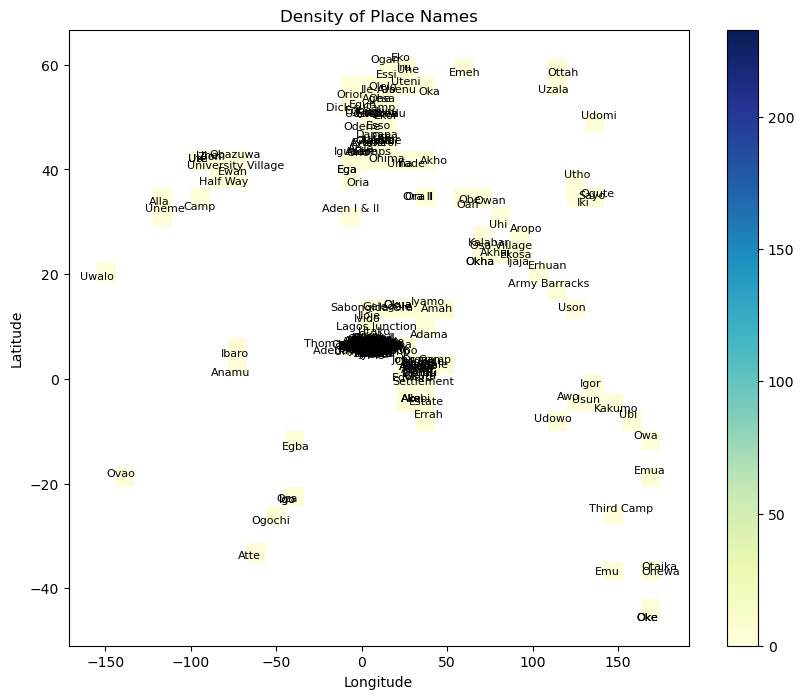
\includegraphics[width=1\linewidth]{heatmap1.png}
    \caption{Heat map presenting the density of place names}
    \label{fig:heatmap}
\end{figure}

The heat map, as shown in Figure~\ref{fig:heatmap}, was generated using a Python script that utilizes the collected data to visualize the density of historical place names. This visualization can be used in further research to identify areas with significant historical importance and understand regional naming patterns.

\begin{figure}[H]
    \centering
    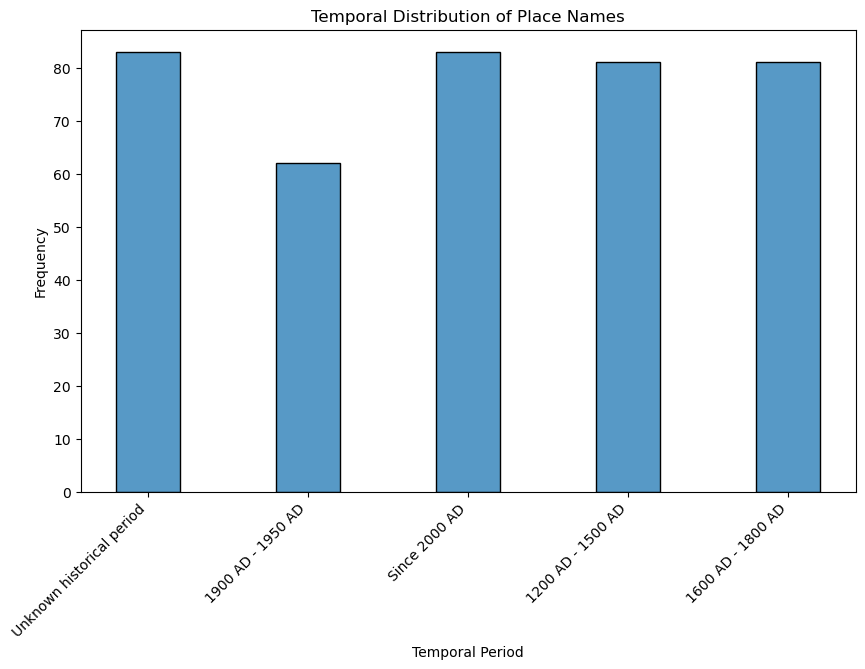
\includegraphics[width=1\linewidth]{output2.png}
    \caption{Temporal Distribution of Place Names}
    \label{fig:histgram}
\end{figure}

The temporal distribution histogram provides insight into the frequency of place names across various historical epochs. The dataset is organized into distinct temporal periods, with each bar representing the count of place names associated with a particular timeframe. By analyzing the distribution of bars, temporal patterns and trends in place-naming practices can be discerned, identifying periods of heightened activity or significance in naming places. This visualization provides the historical context of place names, shedding light on the evolution and dynamics of naming conventions over time.

\begin{figure}[H]
    \centering
    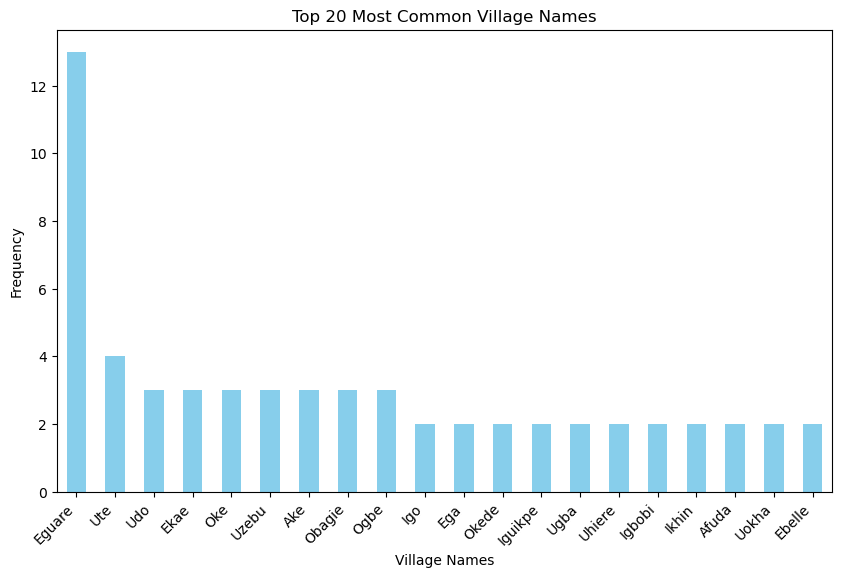
\includegraphics[width=1\linewidth]{histogram2.png}
    \caption{Top 20 Most Common Village Names}
    \label{fig:histogram2}
\end{figure}

The histogram above shows the top 20 most prevalent village names and their frequency in the dataset. It provides a quick insight into common naming trends by displaying the frequency and distribution of village names in the dataset.

\begin{figure}[H]
    \centering
    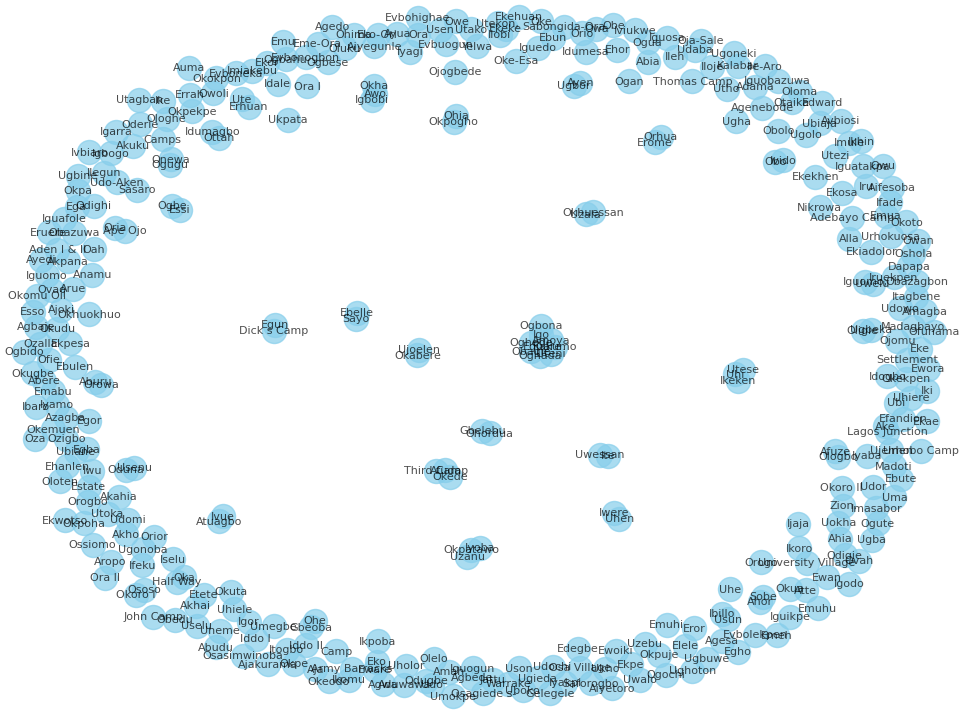
\includegraphics[width=1\linewidth]{networkanalysis.png}
    \caption{Spatial Relationships between Place Names}
    \label{fig:network}
\end{figure}

The spatial relationships between place names, depicted in Figure~\ref{fig:network}, were generated using a Python script. This network visualization helps explore the connectivity and relationships between place names based on proximity or connectivity. This can be useful in further research to understand the social or cultural networks that influenced naming practices.

\begin{figure}[H]
    \centering
    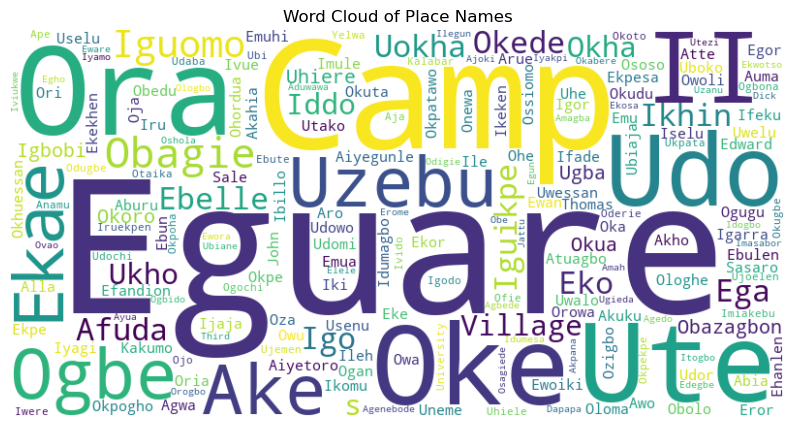
\includegraphics[width=1\linewidth]{wordcloud.png}
    \caption{Word Cloud of Place Names}
    \label{fig:wordcloud}
\end{figure}

The word cloud in Figure~\ref{fig:wordcloud} was also generated using a Python script. This visualization shows the frequency or prevalence of terms in place names, identifying recurring themes or patterns in naming conventions.

\textbf{Ancient Chronicles:} The investigation of ancient chronicles, such as the "Ife Chronicles" and the "Benin Chronicles," offered foundational accounts of early settlements, legendary narratives, and dynastic histories ~\cite{otterbein1966}. According to these chronicles, early settlements were established by legendary figures imbued with divine or semi-divine attributes, signifying their foundational roles in shaping the social and political landscapes of Edo/Benin City. Legendary narratives recount the exploits of these mythical progenitors, depicting their interactions with supernatural beings, the establishment of kinship ties, and the founding of sacred sites. Dynastic histories trace the lineage of ruling families and the succession of kingship within the Edo/Benin polity, highlighting key moments of political consolidation, territorial expansion, and cultural innovation. Through a blend of historical fact and mythic symbolism, these chronicles offer insights into the deep-rooted traditions and cultural heritage underpinning the identity of Edo/Benin City.